\documentclass[12pt,a4paper,twoside]{book}

\usepackage[utf8]{inputenc}
\usepackage[english]{babel}

\usepackage[a4paper,inner=3.5cm,outer=2.5cm]{geometry}
\usepackage{parskip}
\usepackage{indentfirst}

\usepackage{algorithm}
\usepackage{algpseudocode}

\usepackage{graphicx}
\usepackage{float}
\usepackage{booktabs}
\usepackage{tabularx}
\usepackage{multirow}

\usepackage{natbib}
\bibliographystyle{ieeetr}
\setcitestyle{super,open={[},close={]}}

\usepackage{hyperref}

\usepackage{amsmath}
\usepackage{bm}

\usepackage[titletoc,title,toc,page]{appendix}
\usepackage{chngcntr}
\counterwithin{table}{chapter}
\usepackage[capitalize,noabbrev]{cleveref}

\usepackage{newlfont}
\usepackage{fancyhdr}
\usepackage{soul}
\usepackage{xcolor}
\usepackage{hyphenat}
\hyphenation{mate-mati-ca recu-perare}

\usepackage{listings}
\usepackage{verbatim}

\usepackage{tikz}
\usepackage{lscape}

\usepackage{tcolorbox}
\tcbuselibrary{skins, breakable}

\usepackage{enumitem}
\setlist[itemize]{noitemsep, topsep=0pt}
\setlist[enumerate]{noitemsep, topsep=0pt}

\usepackage{amssymb}

\usepackage[font=footnotesize,labelfont=bf]{caption}

\newcommand{\rom}[1]{\uppercase\expandafter{\romannumeral #1\relax}}

\usepackage{pdfpages}

\lstset{
  aboveskip=1em,
  breaklines=true,
  captionpos=b,
  escapeinside={\%*}{*)},
  frame=single,
  numbers=left,
  numbersep=15pt,
  numberstyle=\tiny,
  basicstyle=\ttfamily\footnotesize
}

\definecolor{maroon}{cmyk}{0, 0.87, 0.68, 0.32}
\definecolor{halfgray}{gray}{0.55}
\definecolor{ipython_frame}{RGB}{207, 207, 207}
\definecolor{ipython_bg}{RGB}{247, 247, 247}
\definecolor{ipython_red}{RGB}{186, 33, 33}
\definecolor{ipython_green}{RGB}{0, 128, 0}
\definecolor{ipython_cyan}{RGB}{64, 128, 128}
\definecolor{ipython_purple}{RGB}{170, 34, 255}
\definecolor{outputcellbg}{RGB}{248,248,248}

\newtcolorbox{definition}[1][]{
    enhanced,
    breakable,
    colback=white,
    colframe=maroon,
    arc=2pt,
    boxrule=0.8pt,
    left=10pt,
    right=10pt,
    top=8pt,
    bottom=8pt,
    fonttitle=\bfseries,
    coltitle=white,
    title=Definition,
    #1
}

\newtcolorbox{example}[1][]{
    enhanced,
    breakable,
    colback=white,
    colframe=gray,
    arc=2pt,
    boxrule=0.8pt,
    left=10pt,
    right=10pt,
    top=8pt,
    bottom=8pt,
    fonttitle=\bfseries,
    coltitle=white,
    title=Example,
    #1
}

\begin{document}
\pagestyle{empty}
\newgeometry{left=2cm, right=2cm}
\begin{titlepage}
\begin{center}
    {{\Large{\textsc{Alma Mater Studiorum $\cdot$ Università di Bologna}}}}
    \rule[0.1cm]{\textwidth}{0.1mm}
    \rule[0.5cm]{\textwidth}{0.6mm}\\
    {\small{\bf Second Cycle Degree\\
    Artificial Intelligence}}
\end{center}

\vspace{45mm}

\begin{center}
    \textbf{Exercises \\ Introduction to \\ Complexity and Computability}
\end{center}

\vspace{60mm}
\par
\noindent
\begin{minipage}[t]{0.04\textwidth}
~
\end{minipage}
\begin{minipage}[t]{0.4\textwidth}
{{\textbf{Student:}\\
Matteo Canghiari}}
\end{minipage}
\begin{minipage}[t]{0.04\textwidth}
~
\end{minipage}

\vspace{30mm}

\begin{center}
    {\large{\bf Academic Year 2025/2026}}
\end{center}
\end{titlepage}

\restoregeometry

\pagestyle{empty}
\newpage~\newpage
\thispagestyle{empty}

\clearpage
\pagenumbering{arabic}
\pagestyle{plain}

\chapter{Conceptual and mathemetical preliminaries}
\input{}
\label{c_1}

\chapter{Computational model}
\input{}
\label{c_2}

\chapter{Conceptual and mathemetical preliminaries}
\begin{example}[title = Computational task as a function]
    \textbf{Problem}. \\
    Prove that function \textit{minmax} which given (the encoding of) a list of natural numbers $(a_1, \dots, a_m)$ returns both \textit{min} and \textit{max}
    between $a_1, \dots, a_m$ in \textbf{FP}. \vspace{14pt}

    \textbf{Note}. \\
    We solve a computational task as a function not as a decision problem (\textit{language}), since we need a \textit{path} to achieve the solution. \vspace{14pt}

    \textbf{Solution}. \\
    We can describe an algorithmic solution to this problem as follows:
    \begin{itemize}
        \renewcommand{\labelitemi}{}
        \item \textbf{input}: $(a_1, \dots, a_m)$, $m \in N$, $a_i \in N$.
        \item \textbf{output}: $(b,c)$, where $b$ is the \textit{min} between $a_1, \dots, a_m$ while $c$ is the max value of the list.
    \end{itemize} \vspace{14pt}

    \textbf{Pseudocode}.
    \begin{algorithmic}
        \State $min \gets a_1$
        \State $max \gets a_2$
        \For{$i \gets 2$ $\textbf{to } m$}
            \If{$a_i \le min$}
                \State $min \gets a_i$
            \ElsIf{$a_1 \ge max$}
                \State $max \gets a_i$
            \EndIf
        \EndFor
        \State $return(min, max)$
    \end{algorithmic} \vspace{14pt}

    Now we state the \textit{three things} to prove that the algorithmic solution is in \textbf{FP}. Notice, the \textit{three things} correspond to:
    \begin{enumerate}
        \item Determine the total time complexity of every step done in the solution.
        \item Define if intermediate results have a complexity greater or lower than the total one.
        \item Auxiliary functions or operations don't have a time complexity greater than the total one derived.
    \end{enumerate} \vspace{14pt}
    
    $1^{st}$ \textbf{Total number of steps}. \\ 
    We are gonna to take the whole pseudocode and analyze it piece by piece, considering one macro-operation at time. \vspace{7pt}

    $1^{st}$ macro-operation $\rightarrow$ assignment done for $2$ times. 
    \begin{algorithmic}
        \State $min \gets a_1$
        \State $max \gets a_2$
    \end{algorithmic} \vspace{3.5pt}

    $2^{nd}$ macro-operation $\rightarrow$ loop done for $n$ times (it can be described as $n-1$ since the loop starts from $2$ and not $1$,
    but we can already say that it's proportional to $O(n)$).
    \begin{algorithmic}
        \For{$i \gets 2$ $\textbf{to } m$}
        \EndFor
    \end{algorithmic} \vspace{3.5pt}

    $3^{rd}$ macro-operation $\rightarrow$ repeating comparisons and assignments at most $4$ times at each iteration.
    \begin{algorithmic}
        \If{$a_i \le min$}
            \State $min \gets a_i$
        \ElsIf{$a_1 \ge max$}
            \State $max \gets a_i$
        \EndIf
    \end{algorithmic} \vspace{3.5pt}

    $4^{th}$ macro-operation$\rightarrow$ return done $1$ time.
    \begin{algorithmic}
        \State $return(min, max)$
    \end{algorithmic} \vspace{7pt}

    Therefore the pseudocode above executes at most:
    $$ (2 + O(n) \cdot 4 + 1) \in O(n) $$
    We can also state that the complexity of the algorithm is $ \Theta(n)$, since we have to scan the whole list in any circumstance, so it's strictly 
    proportional to $n$. \vspace{7pt}

    $2^{nd}$ \textbf{Intermediate results}. \\
    The only intermediate results are \textit{min} and \textit{max}, not to much designing this algorithm. However, we can notice that the of $min$ and $max$
    are never greater than the length of the input list, in particular: \vspace{1.5pt}
    \begin{itemize}
        \renewcommand{\labelitemi}{-}
        \item $ |min| \leq |a_1, \dots, a_m| \leq n $
        \item $ |max| \leq |a_1, \dots, a_m| \leq n $
        \item $ |i| \leq log(m \in O(m)) $
    \end{itemize} \vspace{1.5pt}
    We are just stressing that all the intermediate results belong to $O(n)$ or, better, have in the worst case a polynomial time complexity. \vspace{7pt}

    $3^{rd}$ \textbf{Auxiliary functions}. \\
    The auxiliary functions are:
    \begin{itemize}
        \renewcommand{\labelitemi}{-}
        \item two comparisons;
        \item assignments done over the index.
    \end{itemize}
    Each instruction can itself be executed in polynomial time, since the only non-elementary instruction doen is the compatison. \vspace{14pt}

    \textbf{Final mark}. \\
    All in all, given the previous three points, we can state that $minmax$ function is bounded by polynomial time execution, and:
    $$ \textit{minmax} \in \textbf{FP} $$
\end{example}

\begin{example}[title = Decision problem about graphs]
    \textbf{Problem}. \\
    If $G = (V,E)$ is a graph, the reachability problem asks to determine, given $u,v \in V$, whether $v$ it's reachable from $u$, namely whether exists 
    a sequence $w_1, \dots, w_n$ of nodes with $u = w_1$, $v = w_m$ and $(w_i, w_{i+1}) \in E$ for every $i \in \{1, \dots, m-1\}$. \vspace{7pt}

    \begin{center}
        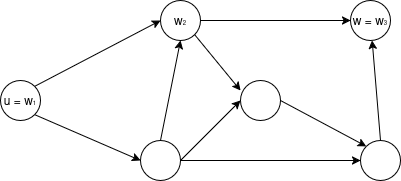
\includegraphics[width = 0.55\textwidth]{img/img1.png}
    \end{center} \vspace{7pt}

    Prove that the above \textbf{decision problem} is in \textbf{P}. \vspace{14pt}

    \textbf{Solution}. \\
    First of all, we define the waited input and the expected output from the algorithmic solution, in particular:
    \begin{itemize}
        \renewcommand{\labelitemi}{}
        \item \textbf{input}: 
        \item \textbf{output}:
    \end{itemize}
\end{example}
\label{c_3}
\end{document}